\documentclass[10pt,halfline,a4paper]{ouparticle}
\usepackage{pgfplots}
\usepackage{amsmath,mathtools,amssymb}
\usepackage{pgf}
\usepackage{graphicx,wrapfig,lipsum}
\usepackage{float}
\usepackage{multirow}
\usepackage{enumerate}
\usepackage{hyperref}
\usepackage{graphicx}
\usepackage{pgfplots}
\usepackage{ragged2e}
\usepackage{adjustbox}
\usetikzlibrary{shapes,arrows,positioning,calc} 
\usetikzlibrary{arrows,chains,positioning,scopes,quotes}
\usepackage{tikz}

\begin{document}
\title{\textbf{Walking Activity Recognition on Smartphone data using Deep Neural Networks}}

\author{%
\small 
\name{Miguel Alba } 
\address{Department of Computer Science, Universität Potsdam\\  Germany}
\email{albaacosta@uni-potsdam.de}
\and
\name{Bostame Md Bayazid}
\address{Department of Computer Science, Universität Potsdam\\  Germany}
\email{bostame@uni-potsdam.de}
\and
\name{Md Shafiul Haque}
\address{Department of Computer Science, Universität Potsdam\\  Germany}
\email{haque@uni-potsdam.de}}

\abstract{
Human activity recognition from sensor readings has proved to be an effective approach in the field of user authentication, smart health care and  many other fields. It is considered to be as one of the complex and challenging tasks due to the fact that human activity is complex and highly diverse. Most of the human daily tasks can be simplified or automated if activity is recognised accurately.This study is intended to contribute to the field of  behavioral biometrics using smartphone's sensor data to determine potential authentication accuracies.The recent advancement of deep learning makes it possible to perform automatic high-level feature extraction thus achieves promising performance in many areas. Since then, deep learning based methods have been widely adopted for the sensor-based activity recognition tasks.In this  study, we are focusing on walking activity recognition, using the data of the motion sensors, such as accelerometer and gyroscope. Data is collected from 25 person that include activities by walking with the smartphone in different positions. Our primary objective is to build a deep neural architecture based on the sensor data in order to predict users activities with the highest possible accuracy. We created a full architecture that we named v7, it is a smaller subset of layers based on VGG16, in this case the network was fed with 3 channel spectrograms, and it was composed by 3 convolutional layers with 3 pooling reductions and 3 final convolutional layers. We added regularization in the first layer (local response normalization), and last fully connected layers with dropouts between 0.5-0.7 including batch normalization.}

\date{\today}

\keywords{Activity Recognition; Deep learning; Sensor data; Convolutional Neural Networks, LSTM}

\maketitle


% \section{Introduction }
%-------------------------------------------------%
%Nowadays world has been in the last years immersed in what it is called the smart device era, in this era dispositives such as smart phones have become in the perfect tool not only for the basic communication but an extension of the human beings in many basic and complex ways. Unfortunately smart phones have not being designed completely with privacy and security. Regarding specifically to the security. All devices count with different forms to authenticate their users with PIN codes, patterns, fingerprints or even facial recognition. Time has been good for different devices to adopt security improvements related to user authentication. Indeed it has been more than ten years since the first phone with fingerprint recognition appeared in the market and few years since the smart phones started to have facial recognition as mandatory. However finding new ways to increase security optimizing the user experience providing smarter phones is a challenge.\\

%\noindent
%As the technology advance providing devices with better capabilities and understanding about the environment and their users, humans become more predictable at the time of provide information to protect their accounts or devices, this has leaded the industry to use user authentication based in what the people have and this is their body instead of passwords and PINs. In fact the end of the passwords has arrived with the use of biometrics as a technology capable of use the human body as a fully connected technological dispositive that can identify the living beings using their biological characteristics. \\

%\noindent
%Biometrics have a wide range of subclasses used for user authentication in mobile devices, most of the smartphone industry has been using fingerprint or facial recognition since 2007 \cite{Thakkar}.  In another hand we might think about behavioral biometrics which data could be measured every time that a user is holding the dispositive in many ways, either holding the phone in different positions, phone typing gestures, swipe gestures or users walking patterns. \\

%\noindent
%Behavioral biometrics are used currently in many applications that varies from fraud detection with identity proofing, continuous authentication and other anomaly detection solutions, according to the International Biometrics Identity Association (IBIA), behavioral biometrics have different properties that make them one of the best ways to provide a proper secure authentication in different cases, this because of the amount of frictionless data points collected and also the continuous authentication provided avoiding the interruption of users experience \cite{IBIA}.\\

%\noindent
%In the case of smartphones, these devices are the perfect way to extract biometric measurements recording behavioral human patterns while they are using them. As a first stage one can think about recognizing a user based on a profile constructed by biometric sensor data, we can predict the user phone activity associated to a sensor mapping and based on these predictions provide a full recognition of the profile for users. Sensors such as accelerometers or gyroscopes are efficient and smaller in almost all devices providing the enough raw data to be processed and analyzed with different algorithms producing a proper user authentication. 


\section{Introduction}

\noindent
Rapid growth of smartphones operating system such as Apple, Android, Microsoft and Blackberry technologies, is changing the nature of interactive computing. Most of the modern devices are embedded with smart sensors, including accelerometer and gyroscope. As a result, peoples’ expectations of use of mobile devices are changing and the vendors are researching on different possibilities to make the interaction and authentication more friendly.\\

\noindent
There has been significant growth in the number and usage of mobile devices in recent years, and this will only continue to grow. Mobile devices are rapidly becoming a key computing platform, transforming how people access business and personal information  \cite{Twewin}.\\

\noindent
User authentication refers to the process in which a user submits her identity credential (often represented by paired username and password) to an information system and validates to the system that she is who she claims to be. In general, there are three types of authentication factors: something a user knows (e.g., a password), something a user has (e.g., a secure token), and something a user is (e.g., biometric characteristics). Passwords are the most common authentication mechanism. However, password-based authentication has many security issues \cite{Klein} \cite{Own} \cite{Ratha}. and is not suitable for wrist worn devices. In general, a biometric authentication system verifies a person based on either his/her physiological traits (e.g., fingerprint, face, voice, iris, bio-impedance, etc.) \cite{Own} \cite{Anzaku} \cite{Cornelius} or behavioral biometrics (e.g., finger or hand movements) \cite{Zheng} \cite{Luca}.\\

\noindent
Behavioral biometrics would be suitable for purposes of authenticating users of smartphones. It will likely be harder for someone with malicious intent to successfully capture a natural motion compared to a password or even a fingerprint. Natural motions also provide the option of continuous authentication since motions such as holding the device, walking around with \cite{Maghsoudi}.

\noindent 
Biometric recognition could be a good alternative to overcoming the difficulties of password and token approaches \cite{Alariki}\cite{Crawford}. These tokens and passwords fail to keep pace with the challenges presented because they can be lost or stolen, which exposes the information \cite{Alariki}. The industry and research have turned their focus in finding a more secure way to authenticate users. Biometrics authentication has, thus, become a interesting topics for academic research and industry adoption/implementation to provide users enhanced security and authentications. Despite it's short comings, Biometric based user authentication will become one of the best approaches that can be used to provide the proper safely of users’ sensitive information as well as ensuring an hassle-free interaction with the system.\\


\noindent
Human Activity Recognition (HAR) has been on of the use-cases where the majority of researchers have started in order to study the possibility of ensure the authentication of users based on behavioral biometrics, in the majority of studies the goal is to predict the majority of activities that individuals make based on sensor data, for these studies we might find some public datasets\\

\begin{table}[ht]
	\begin{adjustbox}{width=1\textwidth}
	\begin{tabular}{|l|l|l|l|l|l|l|l|}
		\hline
		Dataset     & Samples & Persons & Sensors                                            & Associate Task                             & Accuracy & Number of Activities & Sampling Rate \\ \hline
		ActiveMiles & 4390726                  & 10                & A, G & deep learning approach                     & 95.1\%   & 7                    & 50 – 200 Hz   \\ \hline
		WISDM v1.1  & 1098207                  & 29                & A                                   & Artificial features + Dropout              & 85.36\%  & 6                    & 20 Hz         \\ \hline
		RealWorld   & 944,356                  & 15                & A                                   & CNN + statistical features                 & 98\%     & 8                    & 50 Hz         \\ \hline
		HMMwithPre  & 10663                    & 25                & A,G,M,AP  & tacking Denoising Autoencoder and LightGBM & 95.73\%  & 8                    & 100 Hz        \\ \hline
		HSBD        & 10349                    & 30                & A, G                   & tacking Denoising Autoencoder and LightGBM & 98.22\%  & 6                    & 50 Hz         \\ \hline
		HDBD        & 5584                     & 30                & A, G                      & tacking Denoising Autoencoder and LightGBM & 96.31\%  & 6                    & 50 Hz         \\ \hline
		HASC        & -                        & 7                 & A                              & deep recurrent neural network              & 95.42\%  & 6                    & 100 Hz        \\ \hline
	\end{tabular}
	\end{adjustbox}
	\caption{Public datasets for HAR, the values (A)ccelerometer, (G)yroscope, (M)agnetic and (AP) Air pressure}
\label{joint_dist} 
\end{table}

\noindent WISDM v1.1 \cite{Jennifer}:  is a standard HAR dataset which is publicly available from the WISDM group. Android smartphone based application was used to collect data. Each subject was asked to carry the smartphone in a front leg pocket and performed five different activities in supervised condition which were walking, jogging, walking upstairs, walking downstairs, sitting, and standing. While performing these activities, the sampling rate for accelerometer sensor was kept of 20Hz. \\

\noindent ActiveMiles \cite{Ravi}: which contains unconstrained real-world human activity data from ten subjects collected using five different smartphones. Each subject was asked to annotate the activities they carried out during the day using an Android app developed for this purpose. There are no limitations on where the smartphone is located (i.e., pocket, bag, or held in the hand). Annotations record the start time, end time, and label of continuous activity. Since each smartphone uses a different brand of the sensor, the final dataset will contain data that have many modalities, including different sampling rates and amplitude ranges. It is one of the largest datasets in terms of a number of samples with around 30 h of labeled raw data, and it is the first database that groups together data captured using different sensor configurations.\\

\noindent The Human Moving Modes with Pressure (HMMwithPre): This dataset is from a variety of smartphones (HUAWEI NXT-TL00, NXT-AL10, Samsung G9200, MIX 2, and MI 5s) positioned horizontally in the user’s hand to collect data from an accelerometer, gyroscope, magnetic, and air pressure sensor at a 100 Hz sampling rate. Twenty-five (25) subjects participated in data collection: 20 men and 5 women from 20| 50 years old, of 165|192 cm height and 48 | 80 kg weight. Let n represents the length of the sequence. The processed data were built from 50\%-overlapping sliding windows with 256 samples. Since the sampling frequency was 100 Hz, each data frame lasted 2.56 s, with every new frame available every 1.28 s. Finally, the sample shape obtained is ((n|128) | 1,256,10).\\

\noindent The Human Static Behavior Dataset (HSBD): This dataset is from a single smartphone (Samsung Galaxy S2) positioned on the user’s waist to collect the total accelerometer, the estimated body accelerometer and gyroscope data at a 50 Hz sampling rate. Thirty (30) subjects aged 19 to 48 years participated in data collection. The processed data were built from no-overlapping sliding windows with 2.56 s. Since the sampling frequency was 50 Hz, each data frame contains 128 samples. Finally, the sample shape obtained is (n|128,128,9)\\

\noindent The Human Dynamic Behavior Dataset (HDBD): This dataset is from a single smartphone (Samsung Galaxy S2) positioned on the user’s waist to collect the total accelerometer, the estimated body accelerometer and gyroscope data at a 50 Hz sampling rate. It is an updated version of the HSBD. After removing the data which has the same label with HSBD, the training samples were extracted. Considering the small number of datasets, a 0.16 s sliding window is adapted to obtain the samples, the shape of which is ((n|8) | 1,128,9).\\

\noindent
The aim of our work is provide a fresh way to see the HAR based on complete new smartphone sensor dataset, in the collected dataset we have classes which are composed from different activities that persons do while walking using actively or passively their smartphones, with this new dataset we want to show if the activity recognition using deep neural networks (specifically Convolutional Neural Networks CNNs) is possible for the classes proposed.\\

\noindent
The use and specification of the model are based on the fact that we can construct representations of the frequencies of sensors in every activity in form of spectrograms and use tools from computer vision such as CNNs to extract relevant features of the frequency representations. The use of CNNs is frequent in the analysis of signals and sound/speech processing. We would like to give you some examples where this have been seen in the last years.

\noindent
In this paper our goal is to present a new approach for recognizing activities and positioning of the smart phone while walking, with a new dataset that has not been seen in studies of the same characteristics. 
\begin{itemize}
	\item We have the data of 30 users that was taken in a simulated environment, the activities or situations that were collected contain states related to the interaction of the individuals with the phone texting, reading, telephoning and device places for the device while walking, the data was taken in a first study \cite{Klieme} which aim was create a system that verified user identity based on several real world smartphone placements and yet not regarded interactions while walking. 
\end{itemize}


\section{Related work}

As mentioned before, many authors have approach the subject of human activity recognition and verification in many ways, some of them using deep neural networks for continuous authentication using autoencoders based on sensor data adapting to the behavior of users, techniques with the objective of detecting anomalies \cite{Parreno}, other authors have suggest similiar workflows with datasets related to HAR in order to classify activities, that is the case of \cite{Ravi} which proposed a temporal convolutional neural network that was able to identify in different pre-arrenged spectrograms with the accelerometer and gyroscope data different activities, A human activity recognition technique based on a temporal convolution on the spectrogram domain of the inertial data that the learned features are invariant to changes in different properties is designed to enable accurate and real-time classification for low-power wearable devices.
 \cite{Ravi}. \\

\noindent
There are other authors which  have opted for other architectures such as auto encoders to describe and extract the different features to sanitize the noise of sensors \cite{Gaos}; another interesting way to analyze similar data was the one proposed by \cite{Ordonez}, which consist in the ensemble between deep constitutional neural networks and LSTM (Long-Short Term Memory)  networks in order to predict activities from two public datasets, the study suggest that adding the temporal dynamics to the spacial low level feature extraction components provided by CNNs was better over 4\% in average with their framework including a RNN assemble.\\

\noindent
\cite{Ugulino} In this paper also presents, a machine learning base HAR classifier for the classification of five different activities (sitting, standing, sitting down, standing up and walking) using body worn accelerometer data gathered from 4 subjects. Best first selection method was performed to select 12 best features for activity classification. Their experimental result demonstrates that the best classification rate of 99.4\% was obtained for C.45 decision tree in connection with AdaBoost. Autoregressive model can also be used to perform activity recognition task.\\

\noindent
\cite{Zabihi} In This other paper performs activity recognition by transforming the accelerometer data $(x, y, z)$ to spherical coordinate system $(r, \emptyset, \theta)$ and extracting features from transformed data. 36 derived features with sliding window approach (8 samples) along with 12 accelerometer readings in spherical coordinates were fed into a multilayer perceptron neural network of 48 hidden layers. The results demonstrate that 99.9\% activity recognition was achieved.

\noindent
As many authors have approached on the topic before with different public datasets for general HAR, we would like to search if some approach using deep neural networks might be beneficial in terms of predictive capacity recognizing the activities that the users make while walking using the proposed dataset.

\noindent
The aim of this work is provide a fresh way to see the HAR based on complete new smartphone sensor dataset, in the collected dataset we have classes which are composed from different activities that persons do while walking using actively or passively their smartphones, with this new dataset we want to show if the activity recognition using deep neural networks (specifically Convolutional Neural Networks CNNs) is possible for the classes proposed.\\

\noindent
The use and specification of the model are based on the fact that we can construct representations of the frequencies of sensors in every activity in form of spectrograms and use tools from computer vision such as CNNs to extract relevant features of the frequency representations. The use of CNNs is frequent in the analysis of signals and sound/speech processing. We would like to give you some examples where this have been seen in the last years.


\noindent
In this paper our goal is to present a new approach for recognizing activities and positioning of the smart phone while walking, with a new dataset that has not been seen in studies of the same characteristics. 
\begin{itemize}
	\item We have the data of 30 users that was taken in a simulated environment, the activities or situations that were collected contain states related to the interaction of the individuals with the phone texting, reading, telephoning and device places for the device while walking, the data was taken in a first study \cite{Klieme} which aim was create a system that verified user identity based on several real world smartphone placements and yet not regarded interactions while walking. 
\end{itemize}

\section{Data Processing}

The data that was extracted of the experiment contain the interaction between the different placements of the phone as well as a the next collection of activities, 7 interaction activities containing reading, texting, watching videos, listening to a voice message, recording a voice message and answering a call other 9 depending on the wearing side and position right or left in (trousers, jacket, backpack, backside pocket and holding in hands) and 3 wearing activities depending on central placements \cite{Klieme}. \\

\noindent
According to the study in which the data was collected the 25 participants used a Google Pixel Smartphone to collect 30 seconds of pure walking per wearing or interaction activity. the sampling configuration for the sensor data extracted posses a sampling frequency with the lowest delay of 400Hz.
In order to process the data we constructed the series equivalent to all of the samples taken by every sensor in the data, this means time series consisting of multivariate values depending on the coordinates of all the sensors taken by the smartphone.

\begin{figure}[H]
	\centering
	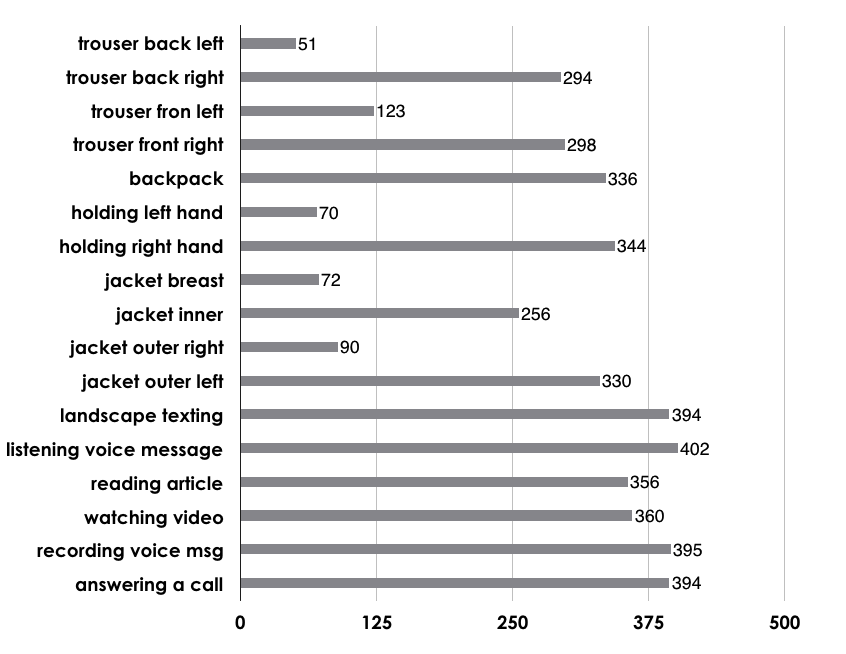
\includegraphics[width=0.6\linewidth]{image_1}
	\caption{Barplot of all the time series in the activities studied}
	\label{fig:image1}
\end{figure}

\noindent
All activities presented in the Table 1, are based on all the different time series for the sensors and different coordinates presented for them, as an example, the accelerometer and gyroscope sensors posses three coordinates which are processes composed in different axes $(x,y,z)$,  all sensors have an specific identifier \cite{google} between 1 and 6 coordinates. The most important sensors for this study are the accelerometer and gyroscope. We have 614 total multivariate $(x,y,z)$ time series for accelerometer and gyroscope distributed among the 18 activities of the study. 

\subsection{Preprocessing}

\noindent
Sensor data can be process to feed machine learning models in many ways, regarding to deep learning architectures, as the easiest approach time series could flow through multilayer perceptrons in a common neural network and predict the different classes proposed, however they may lack the way of the  extraction of low level features in different patterns surrounding the dynamics of the sensor data points. Another way might be use time distributed models such as LSTM networks and Gate Recurrent Units.\\

\noindent
For the purposes of this investigation we investigate the use of convolutiuonal neural networks (CNNs) to extract relevant features of the frequency representation of the sensors in form of spectrograms, to built such representations of the signals, we needed to compute the Short Fourier Transformation (SFT) with the time series  $(x,y,z)$ for the sensors. \\

\noindent
In principle we decided to use spectrograms as some researchers have found that using this synthesized images in problems related with human activity recognition might be of grand benefit, as they represent the energy of the signals in terms of the frequency and amplitude over time; also other studies have found promising results in signal processing and speech recognition using spectrogram data \cite{Parreno} \cite{Ravi} \cite{Ordonez}. \\

\noindent 
In order to build the spectrograms we decided to use the Fourier transformation and the power of the spectrum for the signal coordinates presented in the data, which allow to see the perturbations of the signal in terms of frequency over the time, this transformation has the following form:
\begin{align}
x(t) = \int_{-\infty}^{\infty}{f(x)e^{-2\pi jx} dx}
\end{align} 
for any $x\in \mathbb{R}$. This transformation can be used to compute the frequency of the spectrum in  $N$ points based on a windowing, and then compute the power of the spectrum (periodogram) using the following equation:
\begin{align*}
P = \frac{|FFT(x_i)|^2}{N}
\end{align*}
Where $N$ is also known as NFFT and it is typically around 256, 512, $x_i$ is the $i^{\text{th}}$ frame of the signal $x$. \cite{speech}\\

\noindent
Based on the periodograms we can construct apply filter banks, which is a technique frequently used in audio processing computing triangular filters on a mel-scale in order to stract frecuency bands, we used in our experiments a total of 50 of these triangular filters in order to preserve the consistency of the images fed in the models.

\begin{table}[H]
	\centering
	\begin{tabular}{lll}
		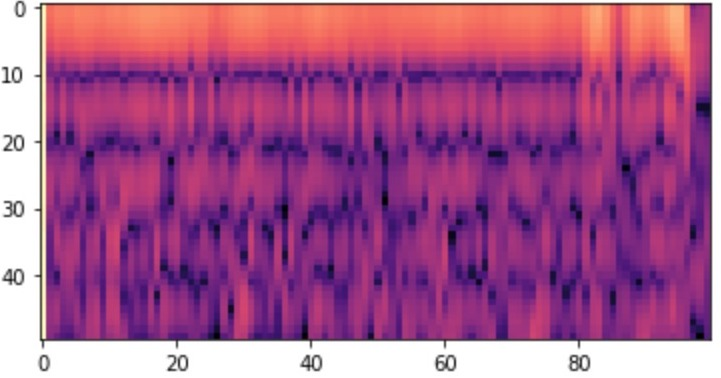
\includegraphics[width=0.3\linewidth]{x} &
		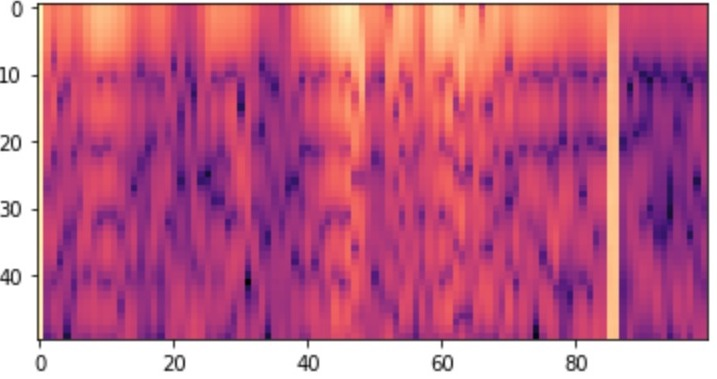
\includegraphics[width=0.3\linewidth]{y} &
		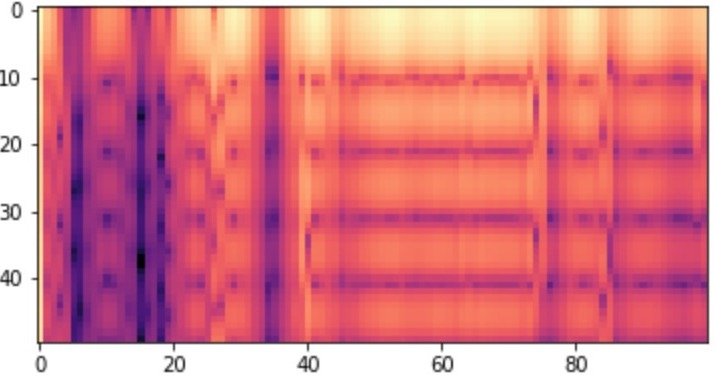
\includegraphics[width=0.3\linewidth]{z}
	\end{tabular}
	\caption{Spectrograms for the coordinates $x$, $y$ and $z$ of one window for accelerometer in Texting activity }
	\label{tab:coordinates}
\end{table}

\noindent
we can see in the constructions of these spectrograms that height is related to the number of triangular filters, and width is related to the amount of samples used to compute the FFT, for this investigation we used in principle 203 and 406 to generate 50 and 100 width spectrograms respectively (Table 2). The sampling rate to create this images was the original used in the recollection of the data (400Hz). \\


\noindent
In principle using single variable spectrograms was the baseline for the experiments, as every image consisted of showing the variability of signals in terms of pixel intensities. Then we were able to fed a CNN with the raw representations (one channel images) and lately the construction of 3 channel images based on the stacks generated every window for $x$, $y$ and $z$ using accelerometer and gyroscope data in order to keep consistency. With these last built preprocessed images we ensured that the model could learn the low level representations in every instant based on a three dimensional space input and make it able to discriminate better the activities based on the idea that different perturbations might affect the sensors while walking in every direction of the coordinates at every time.\\

\begin{figure}[H]
	\centering
	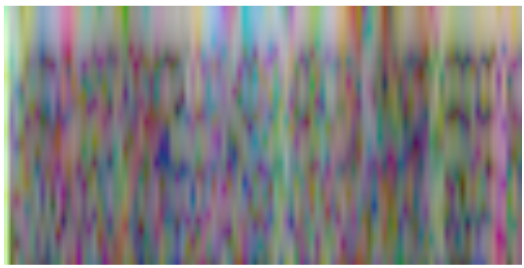
\includegraphics[width=0.3\linewidth]{3channel}
	\caption{3-Channel spectrogram constructed with $x$, $y$ and $z$}
	\label{fig:3channel}
\end{figure}


\noindent
This means if a person is walking and the network aims to discriminate the activities, it would be more useful to the network to be trained using all the data provided by the accelerometer and gyroscope in $x$, $y$ and $z$ at the time $t$.

\begin{figure}[H]
	\centering
	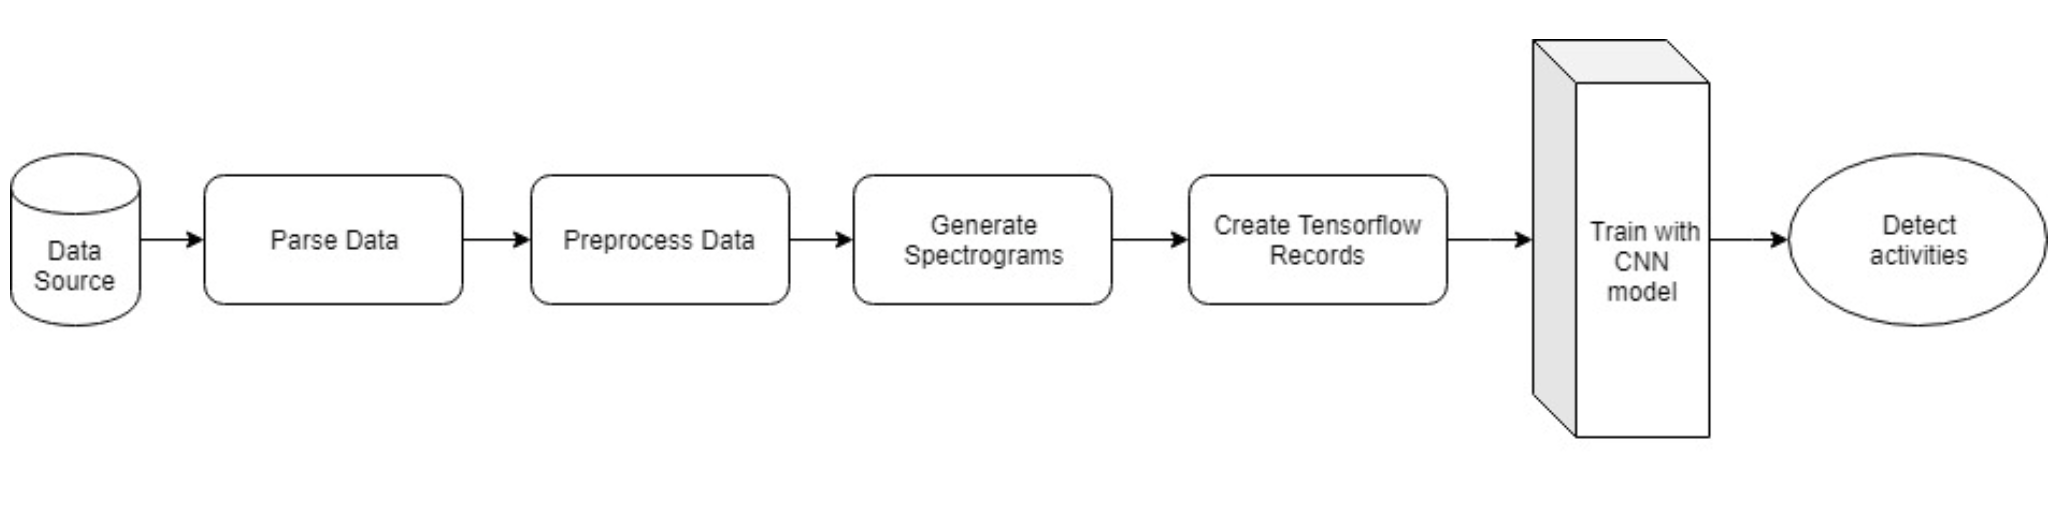
\includegraphics[width=0.7\linewidth]{mlpipeline}
	\caption{Machine learning pipeline}
	\label{fig:mlpipeline}
\end{figure}


\noindent
Preprocess the different experiments cost diverse requirements, in terms of time, single variable spectrograms generation average was among 1 and 1,5 hours approximately depending on the amount  of sensors and activities used, as an example with (2.7 GHz Intel Core i5) the process, creation and stacking to build 3 channel images is around 2 hours.\\

\noindent
For the creation of the architecture we used Tensorflow as the main framework and based on the different amount of images generated (between 18.000-1.500.000 depending on the experiment) we used input pipeline performance in order to increase the workflow between prototyping and model tuning using TFrecords, the generation of these sequences of binary strings was used after preprocessing the data and allowed us to split it using diverse strategies. In the different experiments we created several attempts to select a proper partition to improve the results, this splitting was implemented at the beginning using 18 persons for training, 2 for testing/validating and leaving out 3 to evaluate the results, finally based on the training sessions we decided to use a more classical splitting taking 70\% of the observations of every activity in every person as training data and leaving 30\% to test/validate, in this last case we conserved the 3 selected evaluation persons of the original splitting.\\

\noindent
We feed the networks to classify the different activities depending on the data configuration used in the preprocessing, in some circumstances we fed the model using 18 activities and all sensors as well as one channel spectrograms, then another preprocessings decreasing the subset of activities based on a threshold in the number of observations and using one and three channel spectrograms, the best results were found classifying 10 distinguishable activities.
\begin{table}[H]
	\centering
	\begin{tabular}{|l|l|}
		\hline
		& Activity \\ \hline
		1 & Phone in Backpack \\ \hline
		2 & Holding in right hand \\ \hline
		3 & Jacket outer left \\ \hline
		4 & Text landscape \\ \hline
		5 & Text portrait \\ \hline
		6 & Listening voice message \\ \hline
		7 & Recording voice message \\ \hline
		8 & Reading article \\ \hline
		9 & Watching a video \\ \hline
		10 & Telephoning \\ \hline
	\end{tabular}
	\caption{Important activities selected based on the amount of sensor time series}
	\label{tab:my-table}
\end{table}

\noindent
Moreover we picked these 10 activities taking into account the ambiguity present in the noise of the spectrograms, this given the fact that some activities are similar to others and very difficult to discriminate one of each other, as an example holding the phone with the left hand and holding the phone with right hand. 

\section{Deep neural networks}

\noindent
After preprocess the data and generate the proper input pipeline, we built a convolutional neural network with the next parameter configuration\\

\begin{figure}[H]
	\centering
	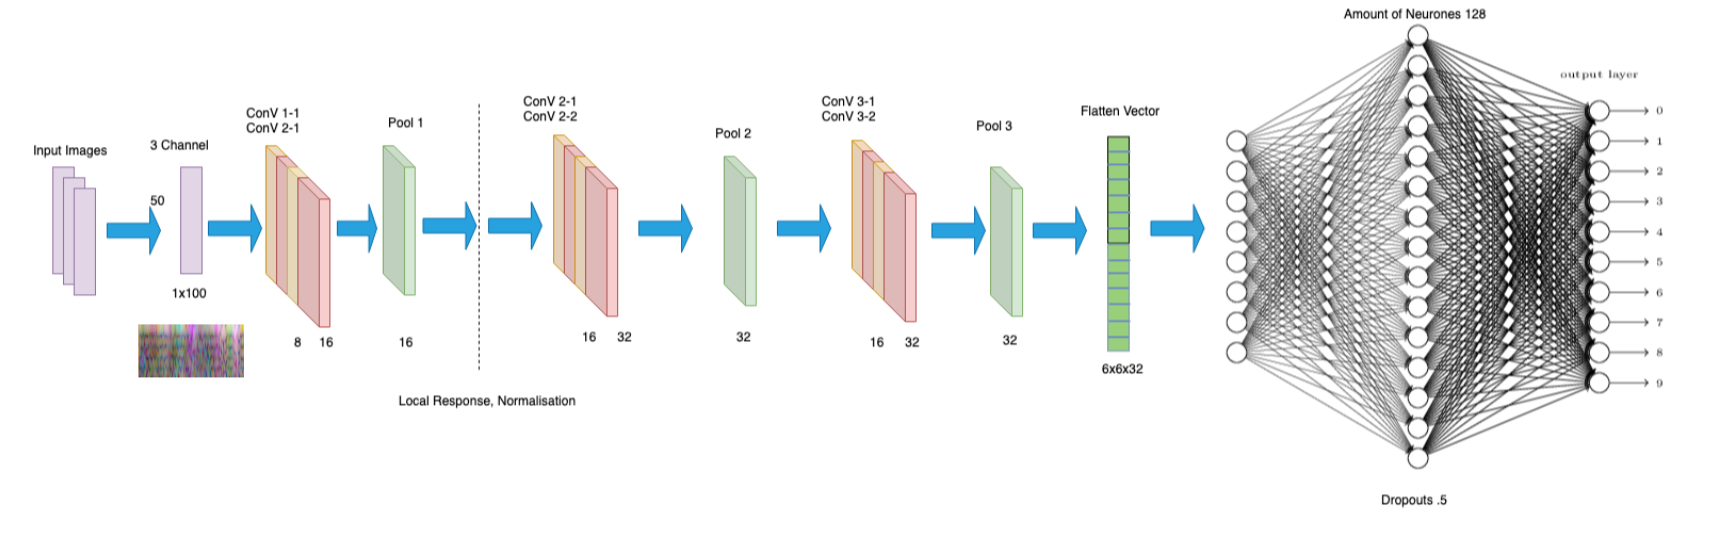
\includegraphics[width=0.9\linewidth]{small_sence}
	\caption{Convolutional Neural Network "small scence v7"}
	\label{fig:smallsence}
\end{figure}

\noindent
 In our case the patterns are imperceptible for human sight, therefore we used a network adapted to detect low level representations caring about the overffiting and architecture complexity. This architecture is based on a subset of weights and layers of VGG 16 structure, it consist of three different convolutional layers, three dimensional max pooling reductions after every one of them and at the end a fully connected layer with one hidden layer.\\

\noindent
We tried to make the CNN architecture consistent in the amount of layers as well as in regularizations based on the abstract representations found in the images that we created, therefore in the first layer we used local response normalization and batch normalization with dropout in the last layers. \\

\noindent
Due to the complexity and the run time of the experiments our goal in the investigation was focused on the way to reach a proper architecture definition and hyperparameters, therefore our results are based on the training sessions that we performed with several data configurations, we found in different trials that increasing the layers as well as dropout in fully connected decreased the accuracy and performance in terms of loss. \\

\noindent
In terms of hyperparameters and solver, using Adam as the main optimizer with a low learning rate (0.0001 to 0.001) improve the results compared to the common stochastic gradient descend, we used also a modified version of the Adam optimizer with weight decay, which was not good in the majority of experiments varying the penalization from 0.01 to 0.3. In general we have the next main experiments implemented, all of the were performed in a NVIDIA GTX 980\\

\begin{table}[H]
	\centering
	\begin{tabular}{|l|l|l|}
		\hline
		Data configuration & Accuracy & Training Loss \\ \hline
		18 activities, all sensors, one channel 50x50 spectrograms, & 0.345 (tr) |  0.183 (t) & 2.224 \\ \hline
		\begin{tabular}[c]{@{}l@{}}10 activities selected, accelerometer + gyroscope,  \\ 1 channel 50x50 spectrograms\end{tabular} & 0.532(tr) | 0.210 (t) & 1.972 \\ \hline
		\begin{tabular}[c]{@{}l@{}}10 activities selected, accelerometer + gyroscope, \\ 3 channel 50x50 spectrograms, with out normalization\end{tabular} & 0.843 (tr) | 0.304 (t) & 0.4827 \\ \hline
		\begin{tabular}[c]{@{}l@{}}10 activities selected, accelerometer + gyroscope, \\ 3 channel 50x100 spectrograms, with normalization\end{tabular} & 0.741 (tr) | 0.281 (t) & 0.8067 \\ \hline
		\begin{tabular}[c]{@{}l@{}}10 activities selected, accelerometer + gyroscope\\ 3 channel 50x100 spectrograms, with out normalization, \\ decreasing noise of the recordings\end{tabular} & \textbf{0.906 (tr) | 0.467 (t)} & 0.1916 \\ \hline
	\end{tabular}
	\caption{Most relevant data configurations used with training (tr), test/validation (t) accuracies and training losses.}
	\label{tab:my-table}
\end{table}

\noindent
At the worst scenario presented using all the data at once showed the worst performance. We also noticed that our guess about using 3 channel images increased accuracy level in the majority of  experiments. In the last and best data configuration we tried to decrease the noise of the images dropping observations related to the first and last moments of the experiment recording, i.e sampling the data related to the pure activity in the and leaving out tail observations related to the start and end of the recording, which increase substantially the training scores compared to the beginning. Summed to the data preprocessing we used also a bigger regularization of 0.7 in the last fully connected layers and the double of average iterations used in all the experiments, in this experiment 18.000.  \\

\section{Conclusions and future work}
%decreasing the partial noise of the observations leaving out the truly behavior of the signal might increase the quality of the time series, this can be implemented
\noindent
Given the results in the different data configurations and architectures proposed in this investigation, we found that with the correct noise decrease in the observations present in the spectrograms and proper regularization, the activity recognition might still be possible for this set of new classes, there are many ways to improve the quality of results based on spectrograms for this set of activities, starting with preprocessing, decreasing the amount of ambiguous classes or similar activities might help with the generalization of the model, i.e dropping similar activities might increase the way in which the network discriminate between the different classes, another possible experiment might be using a different configurations for the creation of the spectrograms increasing the length of the image generated, this may allow the images to conserved more patterns and then let the network to improve the automatic feature selection process. \\

\noindent
Regarding to the architecture, one way might be the possibility of using ensemble architectures that relate the temporal and spatial component in the spectrograms generated, as we showed in the experiment the images were fed inside of the network not being linked one to each other with more than the label. Using a network capable of link the temporal patterns may increase the performance. \\


\begin{thebibliography}{999}
	\bibitem{Twewin}
	S. Trewin, C. Swart, L. Koved, J. Martino, K. Singh, and S. Ben-David, “Biometric Authentication on a Mobile Device: A Study of User Effort, Error and Task Disruption” from Annual Computer Security Applications Conf., Orlando, FL, 2012, pp. 159-168.
	\bibitem{Maghsoudi}
	J. Maghsoudi and C. C. Tappert, "A Behavioral Biometrics User Authentication Study Using Motion Data from Android Smartphones," 2016 European Intelligence and Security Informatics Conference (EISIC), Uppsala, 2016, pp. 184-187
	\bibitem{Klein}
	D. V. Klein. Foiling the cracker: A survey of, and improvements to, password security. In Proc. the 2nd USENIX Security Workshop, pages 5–14, 1990.
	\bibitem{Own}
	H. S. Own, W. Al-Mayyan, and H. Zedan. Biometric-based authentication system using rough set theory. In Proc. the 7th Intl. Conf. on Rough sets and current trends in computing, RSCTC’10, pages 560–569, 2010.
	\bibitem{Ratha}
	N. Ratha, J. Connell, and R. Bolle. Enhancing security and privacy in biometrics-based authentication systems. IBM Systems Journal, 40(3):614–634, 2001.
	\bibitem{Anzaku}
	 E. T. Anzaku, H. Sohn, and Y. M. Ro. Privacy preserving facial and fingerprint multi- biometric authentication. In Proc. the 9th Intl. Conf. on Digital watermarking, IWDW’10, pages 239–250, 2011.
	\bibitem{Cornelius} 
	C. Cornelius, R. Peterson, J. Skinner, R. Halter, and D. Kotz. A wearable system that knows who wears it. In Proc. MobiSys ’14, pages 55–67, 2014.
	\bibitem{Zheng} 
	 N. Zheng, A. Paloski, and H. Wang. An efficient user verification system via mouse movements. In Proc. the 18th ACM Conf. on Computer and communications security, CCS ’11, pages 139–150, 2011.
	\bibitem{Luca} 
	A. De Luca, A. Hang, F. Brudy, C. Lindner, and H. Hussmann. Touch me once and i know it’s you!: Implicit authentication based on touch screen patterns. In Proc. CHI ’12, pages 987–996, 2012.
	\bibitem{Alariki}
	 A. A. Alariki, and A. A. Manaf, “Biometrics Authentication Using TouchBased Gesture Features for Intelligent Mobile Devices,” in 1 st Int’l Conf. of Recent Trends in Information and Communications Technologies, Johor, Malaysia, 2014, pp. 528-538.
	 \bibitem{Crawford}
	H. Crawford, “Keystroke Dynamics: Characteristics and Opportunities,” in Int’l Conf on Privacy Security and Trust (PST), Ottowa, Canada, 2010 pp. 205-212.
	\bibitem{Parreno}
	Parreno-Centeno, Mario \& van Moorsel, Aad \& Castruccio, Stefano. (2017). Smartphone Continuous Authentication Using Deep Learning Autoencoders. 147-1478. 10.1109/PST.2017.00026. 
	\bibitem{Ravi}
	D. Ravi, C. Wong, B. Lo and G. Yang, "Deep learning for human activity recognition: A resource efficient implementation on low-power devices," 2016 IEEE 13th International Conference on Wearable and Implantable Body Sensor Networks (BSN), San Francisco, CA, 2016, pp. 71-76.
	doi: 10.1109/BSN.2016.7516235,
	\url{URL: http://ieeexplore.ieee.org/stamp/stamp.jsp?tp=\&arnumber=7516235\&isnumber=7516211}
	\bibitem{Gaos}
	Xile Gao 1 , Haiyong Luo 1 , Qu Wang 2 , Fang Zhao 3, Langlang Ye 1 and Yuexia Zhang 4
	1, (2019), A Human Activity Recognition Algorithm Based on Stacking Denoising Autoencoder and LightGBM, MDPI
	\bibitem{Ordonez}
	Javier Ordóñez, Francisco \& Roggen, Daniel. (2016). Deep Convolutional and LSTM Recurrent Neural Networks for Multimodal Wearable Activity Recognition. Sensors. 16. 115. 10.3390/s16010115. 
	\bibitem{Ugulino}
	Ugulino, Wallace, et al.” Wearable computing: accelerometers data classification of body postures and movements.” Advances in Artificial Intelligence-SBIA 2012. Springer Berlin Heidelberg, 2012. 52-61
	\bibitem{Zabihi}
	Zabihi, Samad, PouyanNasrollahi, and Mohammad Bazmara.” Human Activity Recognition Using Accelerometers Values in Different Coordinate Systems.” World Appl. Program 4.12 (2014): 237-240.
	\bibitem{Klieme}
	Eric Klieme, Christian Tietz \& Christoph Meinel, (2018), Beware of SMOMBIES: Verification of Users based on Activities while Walking, 2018 17th IEEE International Conference On Trust, Security And Privacy In Computing And Communications/ 12th IEEE International Conference On Big Data Science And Engineering
	\bibitem{google}
	Android developers, 2019, Sensor Overview, \url{https://developer.android.com/guide/topics/sensors/sensors_overview}
	\bibitem{speech}
	Haytham Fayek, 2016, Speech Processing for Machine Learning: Filter banks, Mel-Frequency Cepstral Coefficients (MFCCs) and What's In-Between, \url{https://haythamfayek.com/2016/04/21/speech-processing-for-machine-learning.html}
	\bibitem{Jennifer}
	Jennifer R. Kwapisz, Gary M. Weiss and Samuel A. Moore (2010). Activity Recognition using Cell Phone Accelerometers, Proceedings of the Fourth International Workshop on Knowledge Discovery from Sensor Data
%	\bibitem{Thakkar}
%	Thakkar, D. (2018). How Fingerprint Recognition on Next Generation Smartphones Taking a Shift,\url{ www.bayometric.com}\\
%	\bibitem{IBIA}
%	IBIA. (2018). Behavioral Biometrics,1090 Vermont Avenue, NW • 6th Floor Washington, DC 20005.  % 202.789.4452 x1309 \url{ IBIA.org}\\
\end{thebibliography}
\end{document}